\documentclass{article}
\usepackage{amsmath}
\usepackage{breqn}
\usepackage[brazil]{babel}
\usepackage[utf8]{inputenc}
\usepackage{float}
\usepackage[T1]{fontenc}
\usepackage{geometry}
\usepackage{gensymb}
\usepackage{graphicx}
\usepackage{subcaption}

\geometry{
% a4paper,
% total={170mm,257mm},
% left=15mm,
% right=15mm,
% top=5mm,
bottom=15mm,
}

% pip install opencv-contrib-python

\pagenumbering{gobble}

\title{Exercício Programa \#2\\MAC5768 - Visão e Processamento de Imagens}
\date{}

\begin{document}
\maketitle

Neste breve relatório, são descritas estratégias adotadas para processar imagens usando conceitos do domínio da frequência, da árvore de componentes (max-tree) e de morfologia matemática.

\section{Filtragem no domínio da frequência}
A primeira imagem a ser reconstruída é o leopardo da figura \ref{fig:leopard0}. A imagem apresenta ruído periódico, propício para tratamento no domínio da frequência. Ao aplicar a transformada de Fourier e, na função resultante $f$, aplicar as transformadas logarítmica e de escala (\texttt{20*log(1+f)}), se obtém um espectro de frequências com mais contraste, facilitando uma análise visual. Tal espectro é mostrado na figura \ref{fig:spectrum0}. É possível observar que há pequenos pontos brancos uniformemente espaçados ao longo da imagem. Estes são os componentes que gostaríamos de remover. Uma estratégia simplificada para isso é aplicar uma máscara Gaussiana em torno do centro do espectro, mantendo as frequências baixas e apagando as altas. Isso seria equivalente a um filtro passa-baixa. Os resultados para diferentes raios da máscara são mostrados na figura \ref{fig:leopard}. Nota-se que, para raios grandes, ainda há um ruído residual e que, para raios menores, a imagem fica menos nítida pois informações importantes dela são eliminadas. Outra estratégia possível seria filtrar o espectro de fato selecionando os pontos brancos de alta frequência e atribuindo intensidade baixa (preto) a eles.


\begin{figure}[H]
	\centering
	\includegraphics[width=.8\linewidth]{images/leopard_noise_spectrum.png}
	\caption{Espectro do leopardo}
	\label{fig:spectrum0}
\end{figure}

\begin{figure}[H]
	\centering
	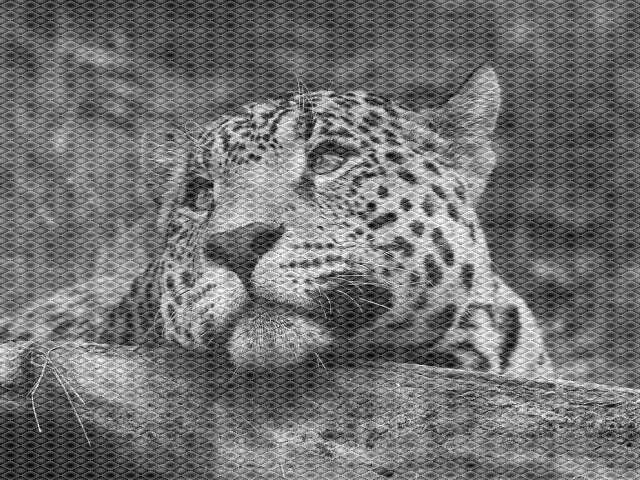
\includegraphics[width=.8\linewidth]{images/leopard_noise.png}
	\caption{Leopardo com ruído periódico}
	\label{fig:leopard0}
\end{figure}

\begin{figure}[H]
	\centering
	\begin{subfigure}{.4\textwidth}
		\includegraphics[width=\linewidth]{images/leopard_noise_filtered_10.png}
		\caption{r=10}
		\label{fig:leopard1}
	\end{subfigure}
	\begin{subfigure}{.4\textwidth}
		\includegraphics[width=\linewidth]{images/leopard_noise_filtered_30.png}
		\caption{r=30}
		\label{fig:leopard1}
	\end{subfigure}
	\begin{subfigure}{.4\textwidth}
		\includegraphics[width=\linewidth]{images/leopard_noise_filtered_60.png}
		\caption{r=60}
		\label{fig:leopard1}
	\end{subfigure}
		\begin{subfigure}{.4\textwidth}
		\includegraphics[width=\linewidth]{images/leopard_noise_filtered_80.png}
		\caption{r=80}
		\label{fig:leopard1}
	\end{subfigure}
	\caption{Filtragem do leopardo com Gaussianas de diferentes raios}
	\label{fig:leopard}
\end{figure}


\section{Remoção de Ruído}
No segundo problema, é dada uma imagem corrompida por um ruído impulsivo, composto de pequenos pontos pretos, conforme mostrado em \ref{fig:fruit0}. A estrutura de dados da árvore de componentes permite que estas regiões sejam podadas de acordo com atributos tais como altura, área e volume. Para podar regiões de mínimo usando o toolbox \texttt{siamxt}, que constrói a max-tree, a imagem de entrada deve ser invertida. Assim, uma poda eliminando ramos com área menor que um dado limite permite eliminar regiões de máximo (equivalentes a pontos brancos). Na figura \ref{fig:fruit}, são mostradas as imagens de saída para diferentes áreas de corte. Observa-se que, escolhendo uma área grande, a intensidade média da imagem cai, indicando que pontos de máximo que continham informação da imagem foram eliminados. O resultado mais adequado foi obtido mantendo os nós com \texttt{area > 12}.

\begin{figure}[H]
	\centering
	\begin{subfigure}{.4\textwidth}
		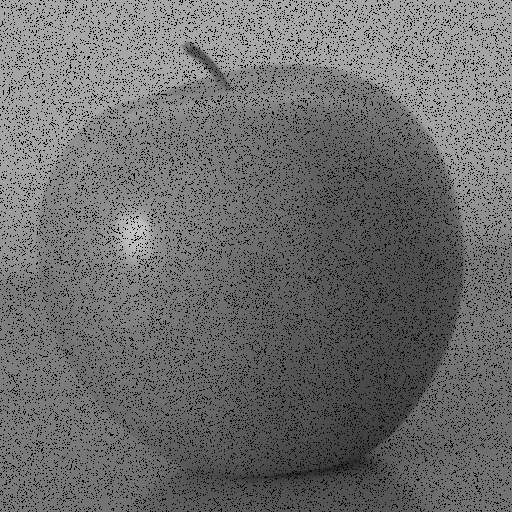
\includegraphics[width=\textwidth]{images/fruit.png}
		\caption{original}
		\label{fig:fruit0}
	\end{subfigure}
	\begin{subfigure}{.4\textwidth}
		\includegraphics[width=\textwidth]{images/fruit_tam8.png}
		\caption{área > 8}
		\label{fig:fruit1}
	\end{subfigure}
	\begin{subfigure}{.4\textwidth}
		\includegraphics[width=\textwidth]{images/fruit_tam12.png}
		\caption{área > 12}
		\label{fig:fruit2}
	\end{subfigure}
	\begin{subfigure}{.4\textwidth}
		\includegraphics[width=\textwidth]{images/fruit_tam16.png}
		\caption{área > 16}
		\label{fig:fruit3}
	\end{subfigure}
	\caption{Fruta com ruído impulsivo}
	\label{fig:fruit}
\end{figure}

\section{Segmentação}
A terceira imagem a ser processada é uma tomografia computadorizada de joelho, mostrada na figura \ref{fig:knee0}. O objetivo do processamento é segmentar a imagem em oito regiões. Para isso, primeiramente, é computado o gradiente morfológico da imagem para detectar as bordas (figura \ref{fig:knee1}). Na saída do gradiente morfológico, é aplicado de um filtro de extinção na max-tree, para manter as oito maiores bacias de acordo com o volume (figura \ref{fig:knee2}). Na imagem obtida pela max-tree, pode então ser feita mais uma filtragem por h bacias ou por extinção pelo atributo de altura. A filtragem de h-bacias é uma reconstrução morfoĺógica superior que usa como J a imagem somada de uma altura h. A filtragem por extinção usa a árvore de componentes para podar os ramos cujos atributos são menores que um dado valor de extinção. Em ambos os casos, as bacias com alturas menores ou iguais a h são preenchidas, e os mínimos regionais são obtidos pela diferença entre a imagem da max-tree e a imagem filtrada. Após computar os mínimos regionais, eles são rotulados para que sejam usados como sementes na entrada da transformada de Watershed. Finalmente, é aplicada a transformada de Watershed na imagem original, resultando na imagem segmentada apresentada na figura \ref{fig:knee3}. Nota-se que o algoritmo foi capaz de selecionar boa parte das regiões que seriam desejáveis. Entretanto, há espaço para melhorias. A qualidade das partições depende da qualidade da imagem, do pré-processamento, da quantidade de partições que foram pré-fixadas e do algoritmo escolhido para marcar as sementes.

\begin{figure}[H]
	\centering
	\begin{subfigure}{.3\textwidth}
		\includegraphics[width=\linewidth]{images/knee_3ch.png}
		\caption{original}
		\label{fig:knee0}
	\end{subfigure}
	\begin{subfigure}{.3\textwidth}
		\includegraphics[width=\linewidth]{images/knee_gradiente_inv.png}
		\caption{gradiente morfológico}
		\label{fig:knee1}
	\end{subfigure}
	\begin{subfigure}{.3\textwidth}
		\includegraphics[width=\linewidth]{images/knee_pos_extincao.png}
		\caption{extinção por volume}
		\label{fig:knee2}
	\end{subfigure}
	\begin{subfigure}{.3\textwidth}
		\includegraphics[width=\linewidth]{images/knee_markers.png}
		\caption{colormap de marcadores}
		\label{fig:knee3}
	\end{subfigure}
	\begin{subfigure}{.3\textwidth}
		\includegraphics[width=\linewidth]{images/knee_with_markers.png}
		\caption{imagem com marcadores}
		\label{fig:knee3}
	\end{subfigure}
	\begin{subfigure}{.3\textwidth}
		\includegraphics[width=\linewidth]{images/knee_result.png}
		\caption{partições de watershed}
		\label{fig:knee3}
	\end{subfigure}
	\caption{Tomografia de joelho}
	\label{fig:knee}
\end{figure}

\section{Detecção de texto}
O último problema tem objetivo de selecionar os caracteres alfanuméricos em preto mostrados na capa de revista da figura \label{revista0}. A abordagem adotada usa filtros morfológicos e árvore de componentes. Para ambas as técnicas, é necessário inverter a imagem, como foi feito no problema 2. Antes de filtrar os caracteres em si, é aplicado um filtro de abertura para eliminar os finos fios de cabelo próximos aos caracteres. O resultado da inversão seguida de abertura é mostrado em \ref{fig:revista1}. Então, é aplicado um filtro usando atributos da max-tree. Foram escolhidos os seguintes atributos: dimensões da bounding box ($dx, dy$), altura ($h$), razão de aspecto ($AR = dx/dy$), razão entre área do objeto e área da bounding box ($RR = area/(dx*dy)$) e variância de cinza ($gray\_var$). Os limiares dos atributos foram definidos empiricamente. Na figura \ref{fig:revista2}, é mostrado o resultado final com as seguintes restrições: \texttt{3 < dx < 65; 15 < dy < 65; h > 10; AR < 2.5; RR > 0.1; gray\_var < 100}.

\begin{figure}[H]
	\centering
	\begin{subfigure}{.45\textwidth}
		\includegraphics[width=\linewidth]{images/revista_fapesp.png}
		\caption{original}
		\label{fig:revista0}
	\end{subfigure}
	\begin{subfigure}{.45\textwidth}
		\includegraphics[width=\linewidth]{images/revista_fapesp_opening.png}
		\caption{inversão e abertura}
		\label{fig:revista1}
	\end{subfigure}
	\begin{subfigure}{.9\textwidth}
		\includegraphics[width=\linewidth]{images/revista_fapesp_filtered.png}
		\caption{caracteres filtrados}
		\label{fig:revista2}
	\end{subfigure}
	\caption{Detecção de texto em revista}
	\label{fig:revista}
\end{figure}

\end{document}
